\chapter{Appendix}%
\label{chap:appendix}

\appendix

\textit{The appendix contains additional information that may help better understand the thesis.\bs}

\chapter*{Complexity Classes}%
Problems in class P have a solution which can be found in polynomial time, problems in \ac{NP} are problems for which no polynomial algorithms have been found yet, and of which it is believed that no polynomial time solution exist. For problems in \ac{NP}, when provided with a solution, verifying that the solution is indeed a valid solution can be done in polynomial time. \ac{NP-hard} problems are a class of problems which are at least as hard as the hardest problems in \ac{NP}. Problems that are \ac{NP-hard} do not have to be elements of NP. They may not even be decidable~\cite{pokharel_computational_2020}. This thesis or other recent studies in the references do not attempt to find an optimal solution. Instead, they provide a solution whilst guaranteeing properties such as near-optimality or probabilistic completeness. As the piano's mover problem can be reduced to the \ac{NAMO} problem combined with relocating objects to target positions, the conclusion can be drawn that this \ac{NAMO} problem is \ac{NP-hard}.\bs

\chapter*{Benchmark Tests}%
 Three benchmark test are presented, the blockade, swap and surround environment, starting with the blockade environment.\bs

In the blockade environment the robot is tasked with placing a box in a target position that is blocked by a cylinder object.\bs
 \begin{figure}[H]
     \centering
     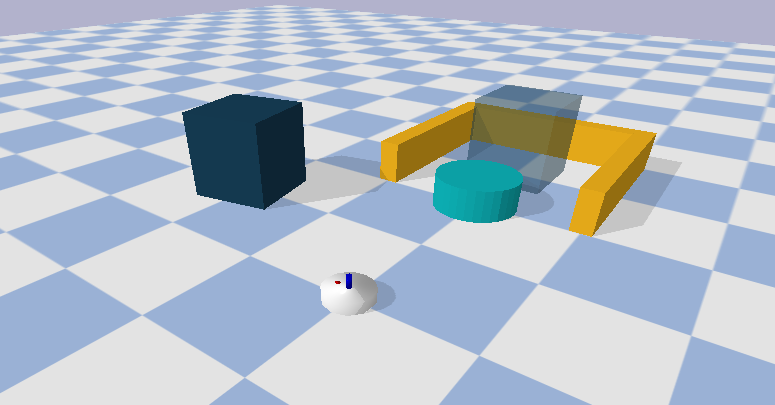
\includegraphics[width=0.9\textwidth]{figures/results/blockade}
     \caption{The blockade environment with the target ghost position for the blue box. The green walls are unmovable whilst both the blue box and cylinder are movable.}%
     \label{fig:benchmark_blockade}
 \end{figure}

In the swap environment the robot should swap the locations of the two objects in the environment.\bs

 \begin{figure}[H]
     \centering
     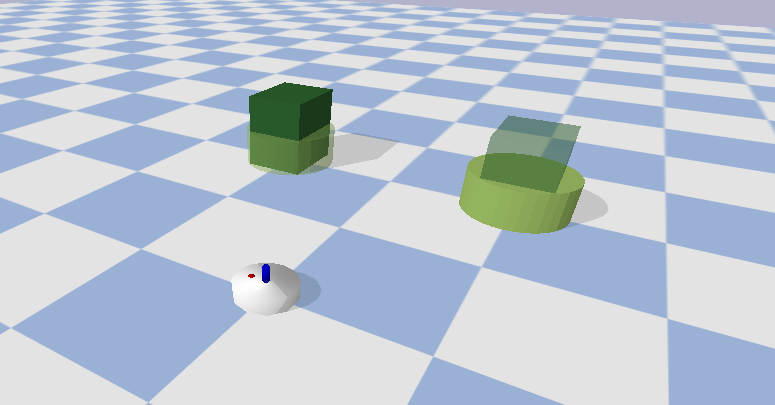
\includegraphics[width=0.9\textwidth]{figures/results/swap}
     \caption{The swap environment, the robot is tasked with swapping the positions of the cylinder and the box.}%
     \label{fig:benchmark_swap}
 \end{figure}

In the surround environment the robot has to learn which box is movable to escape the enclosure of boxes.\bs
 \begin{figure}[H]
     \centering
     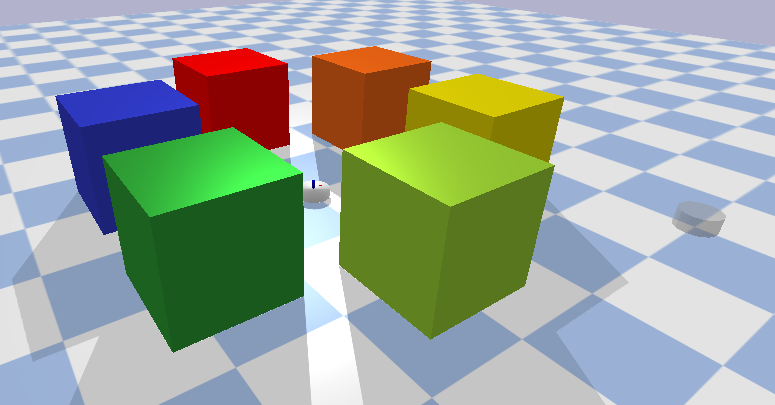
\includegraphics[width=0.9\textwidth]{figures/results/surrounded}
     \caption{The surround environment, the robot is tasked with escaping the surrounding enclosure by driving to the target ghost position displayed on the right side in the figure. Every box objects is unmovable except the red box which is movable.}%
     \label{fig:benchmark_surround}
 \end{figure}

\chapter*{System Models}%
An overview is presented that classifies system models in three categories, analytical-, hybrid- and data-driven models.\bs

\section*{Analytical models}
Historically, analytical models are the first models to emerge, most prominently used are \textit{state-space} representations, \textit{transfer functions} and \textit{differential equations}. Building an analytical model requires thorough knowledge of the system it models, because every system parameter, such as mass, damping coefficient, the center of gravity, geometry, friction coefficient or inertia. Analytical approaches rely on accurate identification of physical parameters which makes analytical models unfit for manipulation while learning system models~\cite{arruda_uncertainty_2017},~\cite{stuber_featurebased_2018}.\\

Nevertheless, the work in~\cite{bauza_dataefficient_2018} manages to create a stable controller for push manipulation using an analytical model. Because thorough model identification of the pushable object was performed, the trajectory error stayed within reasonable boundaries.

\section*{Data-driven models}
Among recent studies, data-driven models shown an uptrend in popularity~\cite{mericli_pushmanipulation_2015,bauza_dataefficient_2018,stuber_featurebased_2018,stuber_let_2020}. Fully data-driven methods don't model any structure of the system it describes, or use a generalised model which applies to all. A system is viewed as a black box, which is fed input and gives back output. This reduces the need for prior information about the system significantly. \ac{IO} data is analysed to estimate the structure of the black box. The \ac{IO} data analysed which solemnly serves the creation of a model is called the \textit{model train set}. The advantage of requiring a minimum of prior information comes at the cost of the amount of \ac{IO} data required. If there is not sufficiently much data, or the data is not rich enough then the model will not be accurate. For example,~\cite{bauza_dataefficient_2018} compared a purely analytical approach with a data-driven approach in push manipulation. The data-driven approach can take up to 200 samples of \ac{IO} data to sufficiently match the performance of an analytical controller. With more \ac{IO} data, data-driven approaches lower output errors and increase performance, outperforming analytical approaches but also outperforming hybrid approaches, which are discussed in the next subsection. Data-driven approaches outperform because data-driven approaches capture even tiny dynamical details of the true dynamics. That is, assuming that the dynamical details reside in the \ac{IO} data. \\

Contact models used for push manipulation make use of robot-object contact or additionally use object-environment contact. With enough rich data contact models outperform analytical and hybrid approaches. To tackle the amount of data required a more hybrid approach is developed. Which separates agent-object contact from object-environment contact. To generate a new model, two things are required, first an object-environment contact model of the object to model, and second, a sufficiently learned agent-object contact model. The latter does not necessarily have to be created from the object to model, existing agent-object contact models, combined with transfer learning can be sufficient~\cite{kopicki_learning_2017}. \\

The nonlinear effects which dominate systems that describe object manipulation reside in \ac{IO} data, because data-driven approaches models are not assuming any structure which could limits capturing nonlinear effects, the data-driven approaches are a worthy method for estimating true dynamics. It must be mentioned that data-driven methods outperform other model classes with enough data, for which the training time is in robotics not always available. If other modelling approaches are available which estimating true dynamics accurate enough, the data-driven approach should be avoided because of the long lasting training time.

\section*{Hybrid models}
Hybrid models are an extension of analytical approaches with data-driven methods. Whilst the interactions between objects are still represented analytically, some quantities of interest are estimated based on observations (e.g. the coefficients of friction)~\cite{stuber_let_2020}. Recent literature reveals the foremost hybrid methods are parameterisable differential equations. Parameterisable state-space models and parameterisable transfer models do exist, though the most widely used parameterisable model remains a parameterisable differential model, which takes the form:
\begin{equation}
   \frac{dx}{dt}=f(x, u, p)
   \label{equation: parameterisable_model}
\end{equation}

where $x$ is the state vector, $u$ is the input vector and $p$ is the parameterisation which needs to be found such that $f(x,u,p)$ accurately estimates the true dynamics. With a random or educated initial guess of the parameterisation $p$, a system model is provided without full knowledge of all system parameters. An initial guess as parameterisation may not be a very accurate model, but it does allow to skip a tedious system identification period. Online adaptation allows to converge to a local minimum during execution. Whether this local minimum also coincides with the global minimum is dependent on the optimisation technique and the initial guess. Parameterisable differential models are very powerful in situations where the general structure of dynamics is known, but certain parameters e.g. weight, the friction coefficient is unknown or change over time~\cite{seegmiller_vehicle_2013}.\\

Single-bodies can and should be modelled as hybrid models, hybrid models allow a workable model which can be created from only the prior structural knowledge of the system. After some off or online system identification detailed parameters can be found, as effect the model will converge toward the true dynamics. While data-driven methods outperforms hybrid methods such methods take long to properly train. Object manipulation models are dominated by nonlinear dynamics, to fully capture such nonlinear dynamics, data-driven methods can and should model manipulation model, even if this means collecting a large train set.

In a environment with unknown objects, the ability to rapidly interact with objects is provided by hybrid models. During interaction hybrid approaches can improve their model accuracy whilst also adapting to changing systems. To fully capture the push mechanics, data-driven methods should be used, because only data-driven methods are able to capture a large portion of the nonlinear dynamics.

\chapter*{Control Methods}%

\section*{\ac{MPC} Control}
In recent literature involving predictive methods \acf{MPC} methods are dominating, before moving on to \ac{MPC} and variations of \ac{MPC}, \ac{MPC} will briefly be explained.  The basic concept of \ac{MPC} is to use a dynamic model to forecast system behaviour and optimise the forecast to produce the best decision for the control move at the current time. Models are therefore central to every form of \ac{MPC}. Because the optimal control move depends on the initial state of the dynamic system~\cite{rawlings_model_2020}. A dynamical model can be presented in various forms, let's consider a familiar differential equation.
$$ \frac{dx}{dt} = f(x(t), u(t)) $$
$$ y = h(x(t), u(t)) $$
$$ x(t_0) = x_0 $$

In which $x \in \mathbb{R}^n $ is the state, $u \in \mathbb{R}^m$ is the input, $y \in \mathbb{R}^p$ is the output, and $t \in \mathbb{R}$ is time. The initial condition specifies the value of the state $x$ at $t = t_0$, and a solution to the differential equation for time greater than $t_0$, $t \in \mathbb{R}_{\geq 0}$ is sought. If little knowledge about the internal structure of a system is available, it may be convenient to take another approach where the state is suppressed, no internal structure about the system is known and the focus lies only on the manipulable inputs and measurable outputs. As shown in \cref{figure: mpc_block_diagam}, consider the system $G(t)$ to be
the connection between $u$ and $y$. In this viewpoint, various system identification techniques are used, in which $u$ is manipulated and $y$ is measured~\cite{rawlings_model_2020}. From the input-output relation, a system model is estimated or improved. The system model can be seen inside the \ac{MPC} controller block in \cref{figure: mpc_block_diagam}.\\

\begin{figure}[H]
\centering
\begin{tikzpicture}
% blocks
\node[draw,
    minimum width=2cm,
    minimum height=1.2cm,
    fill=myLightColor,
] (system) at (0,0){$G(t)$};
\node[draw,
    minimum width=5.5cm,
    minimum height=2cm,
    fill=myEvenLighterColor,
    below = 1cm of system,
    label=above:MPC controller,
] (controller) {};
% the blocks and arrows inside MPC
\node[draw, minimum width=2cm, below=3mm of controller.north, anchor=north, fill=myDarkColor] (optimisation) {Optimisation};
\node[draw, below=8mm of optimisation.south, anchor=south, fill=myDarkColor] (model) {System Model};
\path[-stealth]
        (model.east) edge[bend right=70] node[pos=0.5, right] {Predict} (optimisation.east)
        (optimisation.west) edge[bend right=70] node[pos=0.5, left] {Action}  (model.west);
% Arrows
\draw[-stealth] (controller.west) |- ($(controller.west) - (1,0mm) $) |- (system.west)
node[near end, above]{$u(t)$};
\draw[stealth-] ([yshift=-0.3cm]controller.east) -- ++(3,0) node[midway, above](input){$y_{ref}(t)$, $p$, $\mathbb{X}$, $\mathbb{U}$, $\mathbb{Y}$};
\draw[-stealth] (system.east) -- ++ (5, 0)
    node[midway](output){}node[midway,above]{$y(t)$};
    \draw [-stealth] (output.center) |- ([yshift=0.5cm]controller.east);
\end{tikzpicture}
\caption{System $G(t)$ with input ${u}(t)$, output $y(t)$ and \acs{MPC} controller with input $y(t)$, reference signal $y_{ref}(t)$, parameterisation $p$ and constraint sets $\mathbb{X}$, $\mathbb{U}$, $\mathbb{Y}$} \label{figure: mpc_block_diagam} \end{figure}

Some states of the system might be inside an obstacle region, such a region is undesirable for the robot to be in or go toward. The robot states are allowed in free space, which is all space minus the obstacle region. The free space is specified as a state constrained set $\mathbb{X}$. Allowable input can be restricted by the input constraint set $\mathbb{U}$, a scenario in which input constraints are required is for example the maximum torque an engine produces at full throttle. Lastly, the set of allowed outputs is specified in the output constraint set $\mathbb{Y}$. State, input and output constraints must be respected during optimisation, the optimiser takes the state-, input- and output constraint sets $\mathbb{X}$, $\mathbb{U}$, $\mathbb{Y}$ and if feasible, finds an action sequence driving the system toward the reference signal while constraints are respected. The \ac{MPC} system model predicts future states where the system is steered toward as a result of input actions.\\

The optimisation minimises an objective function $V_{N}(x_{0}, y_{ref}, \mathbf{u}_{N}(0))$, where\\ $ \mathbf{u}_{N}(k) = (u_k, u_{k+1}, \dots , u_{k+N})$. The objective function takes the reference signal as an argument together with the initial state and the control input for the control horizon. The objective function then creates a weighted sum of some heuristic function. States and inputs resulting in outputs far from the reference signal are penalised more by the heuristic function than outputs closer to the reference signal. Because the objective function is a Lyapunov function, it has the property that, it has a global minimum for the optimal input $\mathbf{u}_{N}^*$. If the system output reaches the reference signal $y_{ref}$, $x_{ref}$ then $u_{ref}$ will be mapped to the output reference signal as such $y_{ref} = h(x_{ref}, u_{ref})$. As a result solving the minimisation problem displayed in \cref{equation: mpc_problem} gives the optimal input which steers the system toward the output reference signal while at the same time respecting the constraints.

\begin{mini}
{u_k, u_{k+1}, \dots , u_{k+N}} {
V_{N}(x_{0}, y_{ref}, u_k, u_{k+1}, \dots , u_{k+N})
}
{}{}
\addConstraint{x(k+1) = f(x(k), u(k))}
\addConstraint{x \in \mathbb{X}}
\addConstraint{u \in \mathbb{U}}
\addConstraint{y \in \mathbb{Y}}
\addConstraint{x(0) = x_0}
\label{equation: mpc_problem}
\end{mini}

After solving the minimisation problem, \cref{equation: mpc_problem}, the optimal input sequence is obtained $\mathbf{u}^*_N$ (given that the constraints are respected for such input), from which only the first input is executed for time step $k$ to $k+1$. Then all indices are shifted such that the previous time step $k+1$ becomes $k$, the output is measured and the reference signal, parameterisation, and constraints sets are updated and a new minimisation problem is created, which completes the cycle.\bs

\section*{\ac{MPPI} Control}
\label{sec:appendix_mppi}
Introduced by~\cite{williams_model_2015} \ac{MPPI} control arose. Which was followed by \ac{MPPI} control combined with various system models, identification methods~\cite{abraham_modelbased_2020,cong_selfadapting_2020,arruda_uncertainty_2017}. The core idea is from the current state of the system with the use of a system model and randomly sampled inputs to simulate in the future a number of "rollouts" for a specific time horizon,~\cite{neuromorphictutorial_ltc21_2021}. These rollouts indicate the future states of the system if the randomly sampled inputs would be applied to the system, the future states can be evaluated by a cost function which penalised undesired states and rewards desired future states. A weighted sum over all rollouts determines the input which will be applied to the system. If a goal state is not reached, the control loop starts with the next iteration. An example is provided, see  \cref{figure: mppi_car_with_rollouts}.

\begin{figure}[H]
    \centering
    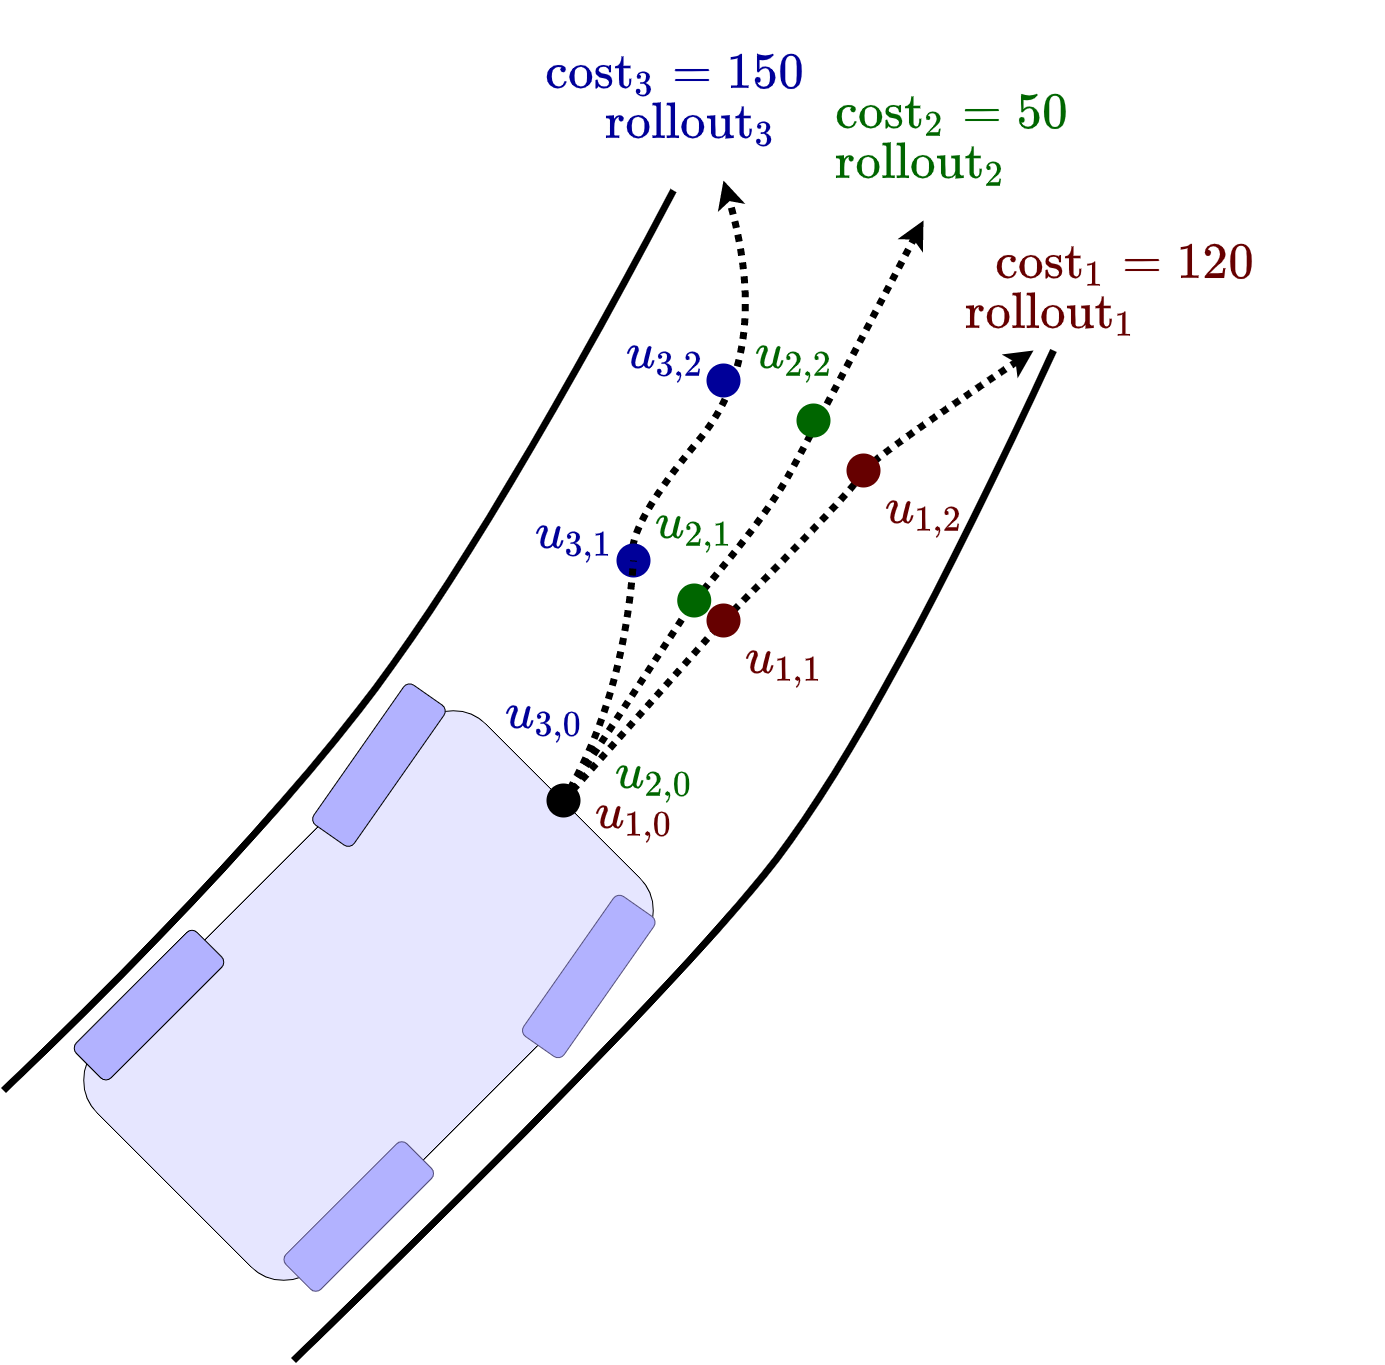
\includegraphics[width=0.3\textwidth]{figures/appendix/MPPI_car_with_rollouts.png}
    \caption{\acs{MPPI} controlled race car using a control horizon of 3 time steps, with 3 rollouts all having their respected inputs as $u_{i,j}$ where $i$ is the rollout index and $j$ indicates the time step~\cite{neuromorphictutorial_ltc21_2021}.}
    \label{figure: mppi_car_with_rollouts}
\end{figure}

Here 3 rollouts are displayed, The objective function is designed to keep the car driving on the center of the road by penalising rollouts which are further away from the center of the road relatively more. resulting in a high cost for $\text{rollout}_1$ and $\text{rollout}_3$ compared to $\text{rollout}_2$. As a result, the input send to the system as a weighted sum of the rollouts is mostly determined by $\text{rollout}_2$. The weighted sum determining the input is displayed in \cref{equation: mppi_weighted_sum}, from~\cite{neuromorphictutorial_ltc21_2021}.

\begin{equation}
u(k+1)=u(k)+\frac{\sum_{i} w_{i} \delta u_{i}}{\sum_{i} w_{i}}
\label{equation: mppi_weighted_sum}
\end{equation}

Where $\delta u_i$ is the difference between $u(k)$ and the input for rollout $i$, the weight of $\text{rollout}_i$ is detemined as: $w_{i}=e^{-\frac{1}{\lambda} \text{cost}_{i}}$, $\lambda$ is a constant parameter.\bs

% \chapter*{Implementation in Python}%
% \label{chap:code_implementation}
%
%
% Code reproducibility in the scientific community is low~\cite{trisovic_largescale_2022}. That is bad, bad bad bad!
%
% \todo[inline]{setup of the system (python version, ubuntu version etc.)}
% \todo[inline]{reference to an install readme file}
% \todo[inline]{Explain what can be changed easily}
% \todo[inline]{Explain code folders (the thingies better to not touch)}

